\chapter{克服拖延症} % Introduction chapter suppressed from the table of contents


技术总监问:现在我遇到最大的难题就是如何提升下面技术人员的能力,如果他们全都是高手,我就很轻松了,但实际上最多只有三分之一,其他都是中低水平。您接触过这么多软件开发团队,有什么好方案?\\
我:可以先听听这故事:\\


= = = = = = = = = = = = = = = = = = = = =


%\href{文件:小李图.png}{400px}


\includegraphics[width=8cm]{小李图.png}

小李:你平常办公时间都一直都很忙,还可以腾出晚上和周末时间,
把客户遇到的问题,如何解决等,汇总成分享文章,每两周公众号发布,很厉害呀。\\
我:其实你也可以做到。要成为专业软件工程师,除了要学习软件工程相关的知识与技能外,
个人有没有高效率的习惯其实更重要。

我在五年前教项目管理时参考过一本效率小册 {[}详见 Reference1{]},
这本小册罗列了99个小技巧,每个技巧都不超过一页纸,我自己也一直用这小手册提醒自己。

%\url{文件:超效率目录.png}

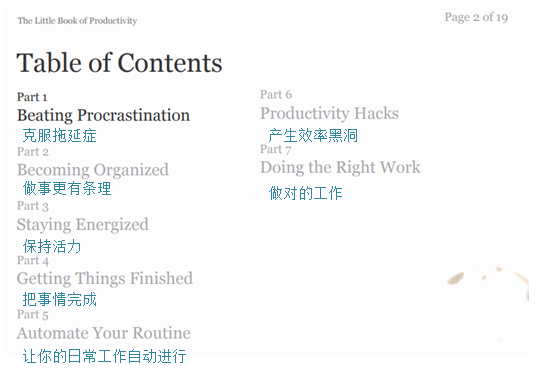
\includegraphics[width=10cm]{超效率目录.png}

例如,第一章``克服拖延症'',这里的几乎全部技巧有帮助:\\

\begin{itemize}
\tightlist
\item
  周 / 日目标 (1 Weekly / daily Goals)
\end{itemize}

\framebox{%
\begin{minipage}[t]{0.97\columnwidth}\raggedright
我每天都会定计划,早上希望完成哪些功能,下午完成哪些。当然这个计划也会按实际的进展调整。

周 /
日目标是个人时间管理的基本功。每一天第一件事不是回邮件,而是仔细想想今天要完成什么任务,每一周的开始,也应该想我本周希望完成什么任务。不然的话,每天的时间就很容易被琐碎的小事吃掉,一事无成。\\
\strut
\end{minipage}}

\framebox{%
\begin{minipage}[t]{0.97\columnwidth}\raggedright
背后的道理很简单, 要把时间花在重要、但非紧急的活动(下图右上角
)上,效率才会出来。

%\href{文件:紧迫非紧迫_3.0.png}{600px}\strut
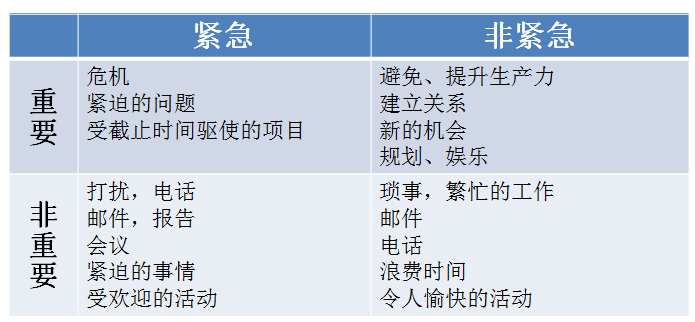
\includegraphics[width=10cm]{紧迫非紧迫30.png}
\strut
\end{minipage}}

\begin{itemize}
\tightlist
\item
  限定时间 (2 Timeboxing)
\end{itemize}

\framebox{%
\begin{minipage}[t]{0.97\columnwidth}\raggedright 把每天的任务安排成时间段,每一段不应超过1.5
小时。\strut 一般人可以专心集中的时间段都不会超过60分钟,小孩可能就更短。如果老师叫你星期五5点钟交卷,你不会3、4点就交,都会等到最后十分钟,甚至五分钟。所以如果我们把一天的时间切开成
1 ~ 1.5 小时时间段,自然有动力,
希望在时间之内完成任务。\strut 我们写代码的时候应该也是用同样的原理。例如。前面那个总共花了10个小时的功能,也是本身尝试了很多次。每次当我发现超过了1小时或者1.5
小时,我就会把它放下来,先做其他事。\strut
\end{minipage}}

\begin{itemize}
\tightlist
\item
  分解任务 (3 Dissolving tasks)
\end{itemize}

\framebox{%
\begin{minipage}[t]{0.97\columnwidth}\raggedright
因为都是练习题,所以每一个功能都比较细,不会超过二十行。如果我们平常做开发时,也必须要把一些大、复杂的功能预先拆分成小的功能才有效率。\strut
\end{minipage}}

\begin{itemize}
\tightlist
\item
  加强自律 (6 Building Self-Discipline Muscles)
\end{itemize}

\begin{description}
\tightlist
\item[]
晨礼(30 Morning Rituals) 日常运动 (32 Make an Exercise Routine)
\end{description}

\framebox{%
\begin{minipage}[t]{0.97\columnwidth}\raggedright
不要以为编码是一个单纯的脑力活。整天坐在电脑前面敲代码就可以,如果人的体力、精力没有配合上也会出问题,好在我每天早上一直坚持三十到四十分钟的轻量运动,然后晚饭前半个小时到一个小时的骑单车或者慢跑的习惯。中间也是不是整天坐着,一段时间会走一走,喝橙汁等,确保身体不断在动,才不会困,保持动力。

贝多芬每天都会去外面散步,来启发一些创作的灵感,然后他会立马把这些写在本子上,用于后面的音乐创作。早上的跑步也可以让我有多些创作灵感。\strut
\end{minipage}}

\begin{itemize}
\tightlist
\item
  不会分心的工作场所 (11 Create a Distraction-Free workplace)
\item
  轻策划,迭代,再策划 (13 Ready , Fire, Aim!)
\end{itemize}

\framebox{%
\begin{minipage}[t]{0.97\columnwidth}\raggedright
三十年前,软件开发都是很大型的一些项目,整个架构要设计好才动手去写代码。现在反过来,需求变化极大,开发都需要敏捷,轻文档轻计划。尽快写好代码,做一些功能给客户,从反馈优化下一轮。我这次的几天开发也是用同样原则,没有花时间在一些设计或者文档。想直接把那个代码写出来,并通过单元测试,就节省很多耗时间的工作。把有限的时间都放在写好代码上。\strut
\end{minipage}}

\begin{itemize}
\tightlist
\item
  不断清洗 (10 Churning)
\end{itemize}

\framebox{%
\begin{minipage}[t]{0.97\columnwidth}\raggedright
万事开头难。我在开始的半天也是遇到同样问题,不知如何入手,太久没看写代码的书了,很多基本的都不知如何入手。所以我开始的时候不会直接尝试写题目里面的功能,而是重写一些书本的代码,看看跑出来怎么样,然后逐步提升。写一些基本功能,慢慢有了习惯,调整过来了,后面就越来越顺。好比一台旧的水泵,刚开始抽上来的水总是有难喝的铁锈,只要不停止抽水,当污水最终都从系统中抽出后,就能发现底下的净水。\strut
\end{minipage}}

\begin{itemize}
\tightlist
\item
  要有好的土壤 (8 Remove your Hidden Roadblocks)
\end{itemize}

\framebox{%
\begin{minipage}[t]{0.97\columnwidth}\raggedright
在含盐量高的土壤里种植物,是结不出果实的。浇水、平衡在阴凉处和阳光下的时间都抵不过根部吸入的毒素。如果我们没有积极性,就可能是土壤的问题。如果没有足够的积极动力,就不会在长假专注写程序,也不会定期要求自己写分享文章。所以要有明确/很想达到的目标驱动。
像一个作曲家,他希望写出很多经典的优秀作品,不满足于现在的状态。觉得自己的灵感或者创造力没有发挥出来,成为可以保留下来的东西。也是这种驱动力让我可以一直努力做这件事。\strut
\end{minipage}}

\begin{itemize}
\tightlist
\item
  摒弃拖延恶习 (14 Quit your Procrastination Vices)
\end{itemize}

\framebox{%
\begin{minipage}[t]{0.97\columnwidth}\raggedright
长假里,大部分人都会把时间用于看视频或电视剧,而我正好没有这个习惯,也一直没有玩网络游戏的习惯,否则肯定完成不了。\strut
\end{minipage}}

最终我用日程记录(91
Timelogging),把整件事和什么活动、时间花在什么地方都记录下来了。

小李:我看你上面列出的技巧,我大部分都还没做到。

我:不要紧,我六年前刚开始定期写文章时情况跟你类似,但只要不放弃,一直往既定目标努力,不良习惯都改正过来了。

我常常说人的潜力是极大的。 舒伯特你听过吗?\\
小李:好像是一个很有名的作曲家。\\
我:是的,但他很年轻31岁(1828)
就去世了,你猜他一生一共写了多少首歌和音乐作品。\\
小李:我记得中学时,老师介绍过他的艺术歌曲,如``鳟鱼 The
Trout'',但他31岁就死了,我猜100 - 200 首歌?\\
我:他一生写了超过460首歌曲(时长\textgreater{}24小时)。除了歌曲,他还写了其他作品,如9首交响曲,20
室内乐,120 钢琴曲等等,每一类都包括大量经典作品,对后世影响深远。\\
小李:如果粗算他一生600作品,算他有16年时间作曲,平均每月要完成3个作品,真是不得了。\\
我:虽然他的作品有大有小(从一首歌,到45分钟的交响曲),他确实生产率极高,而且他最后的7年一直身体都不好,所以他那个时候肯定不会像我们现代996方式工作。
他每天主要是早上用来写作,傍晚便去休息散步。但他会同时做多个创作项目 -
那些项目没有灵感,就暂时放下来,创作其他作品。
他著名的未完成交响曲就是个好例子,只有两个乐章(一般交响曲都是四个乐章)
所以他是使用高效技巧的一个成功例子。

每个人都有自己的理想,但如果没有高效率来执行,理想只是天马行空,天方夜谭,不会有任何成就。有没有疑问?

小李:没有,挺好的,我后面立马就开始。\\
:: = = = = = = = = = = = = = = = = = = = = =\\
总监:我大概懂你的意思了,要提升技术人员的能力先要改变他们的习惯,有良好的习惯(如时间管理),才有机会提升。\\
我:是的。\\
总监:从管理者的角度,我们有什么可以做的?\\

\framebox{%
\begin{minipage}[t]{0.97\columnwidth}\raggedright
即时笔记 (17 The Capture Device)
总监边听边在本子上记下那些重点。高效的人都会有工具帮他记录想到灵感、想法、项目、待做事项等等,不会仅仅靠大脑记忆。你提出一个要求,他会立马写在小本子上,你会觉得他应该会按你要求去处理,但反过来他只是口头说会处理,你会担心很可能没有下文。但我看有些领导,身边只拿个手机,除非他们的记忆力超人,不然话我估计他每天都会忘记不少重要事项。\strut
\end{minipage}}

\hypertarget{ux676dux5ddeux9ad8ux7ea7ux7ecfux7406ux7684ux53cdux9988ux548cux9ad8ux89c1}{%
\subsubsection{杭州高级经理的反馈和高见}\label{ux676dux5ddeux9ad8ux7ea7ux7ecfux7406ux7684ux53cdux9988ux548cux9ad8ux89c1}}

人一定要自律!您说的小技巧确实能起到很大帮助,而且我基本都会使用,但如果不养成习惯,想起来使用下,最终还是改不了拖延症,所以要解决拖延症,一定从根源做起,还是得靠自己,需要培养自己意志力、专注力,坚持好习惯,改掉坏毛病。

\hypertarget{references}{%
\section{References}\label{references}}


1. YOUNG, Scott: "The Little book of Productivity"
(有中文翻译版,叫《超效率手册》 )\\


